\section{Automatic Stream Management Using Program Contexts}

%In developing \textsf{\small PCStream}, our key insight was that in most
%applications, (regardless of their I/O workload characteristics) a few dominant
%I/O activities exist and each dominant I/O activity   represents the
%application's important I/O context (e.g., for logging or for flushing).
%Furthermore, most dominant I/O activities tend to have distinct data lifetime
%patterns.  In order to distinguish data by their lifetimes, therefore, it is
%important to effectively distinguish dominant I/O activities from each other.
%For example, in update workloads, LBAs alone were effective in separating
%dominant I/O activities.  

{\textcolor{blue}{
(TODO: 교수님 검토 필요)
Our key insight in this study is that, in most cases, the overall I/O behaviors of 
applications are decided by a few dominant
I/O activities (e.g., logging and flushing). Moreover, 
data written by dominant I/O activities tend to have unique lifetime patterns.
Therefore, if such dominant I/O activities of applications can be detected or captured,
we are able to effectively distinguish data by their lifetimes.
}}
%(regardless of their I/O workload characteristics) a few dominant
%I/O activities exist and each dominant I/O activity   represents the
%application's important I/O context (e.g., for logging or for flushing).
%Furthermore, most dominant I/O activities tend to have distinct data lifetime
%patterns.  In order to distinguish data by their lifetimes, therefore, it is
%important to effectively distinguish dominant I/O activities from each other.
%For example, in update workloads, LBAs alone were effective in separating
%dominant I/O activities.  

In this paper, we argue that a program context (PC) is an efficient
general-purpose indicator for separating dominant I/O activities.  Here, a PC
represents an execution path of an application which invokes write-related
system call functions such as {\tt write()} and {\tt writev()}.  
There could be various ways of extracting PCs, but the most common approach is to
sum program counter values of all the functions along the execution path which
leads to a \texttt{write()} system call.

%we represent the PC by summing program counter values of
%all the functions along the execution path which leads to a write system call.

\subsection{Distinct Data Lifetime Patterns of Different PCs}

In order to show that using PCs is an effective way to distinguish I/O
activities of an application and data lifetimes, we measure the lifetime
distribution of data written by different PCs for various types of workloads,
including RocksDB~\cite{}, SQLite~\cite{}, and GCC~\cite{}.

In RocksDB, dominant I/O activities include logging, flushing and compaction.
Those are invoked through different function-call paths, so we can easily
identify dominant I/O activities of RocksDB using PCs.  \textcolor{red}{(TODO:
갑자기 Figure 4가 나오는 것이 이상함 $\rightarrow$ Figure 4(a)를 이쪽으로 옮기는
것이 더 좋을 듯...) For example, Fig.~\ref{fig:getpc}(a) shows an execution
path for logging in RocksDB}.  The sum of program counter values of
\texttt{WriteImpl()}, \texttt{WriteToWAL()}, and \texttt{AddRecord()} is used
to represent a PC for the flushing activity. \textcolor{red}{(TODO: 갑자기
lifetime 이야기가 나옴. 없애도 큰 문제가 없을 듯...) \sout{Note that using a
program context to distinguish data lifetimes is not new. For example, Ha {\it
et al.} proposed a data separation technique based on the program
context~\cite{PCHa}.  However, their work was neither designed for append-only
workloads nor for modern multi-streamed SSDs.}}

\begin{figure}[t]
\centering
\hfill
%\vspace{-10pt}
	\subfloat[Logging (PC)]{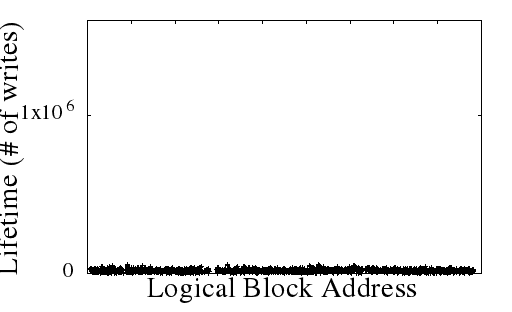
\includegraphics[width=0.2\textwidth]{figure/type_1}} % data from 4/03031953 
	\hspace{2pt}
	\subfloat[Logging (manual)]{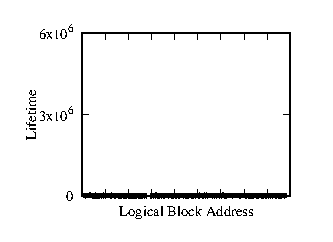
\includegraphics[width=0.2\textwidth]{figure/pcID_2}}
\hfill
\vspace{7pt}
	\subfloat[Flushing (PC)] {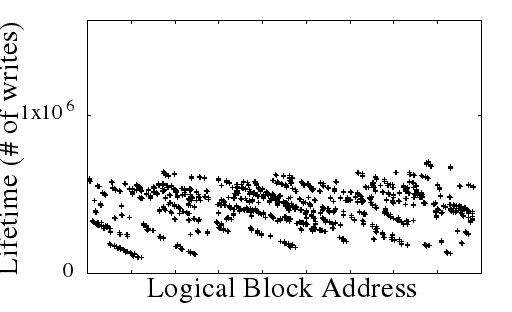
\includegraphics[width=0.2\textwidth]{figure/type_3}}
	\hspace{2pt}
	\subfloat[Flushing (manual)]{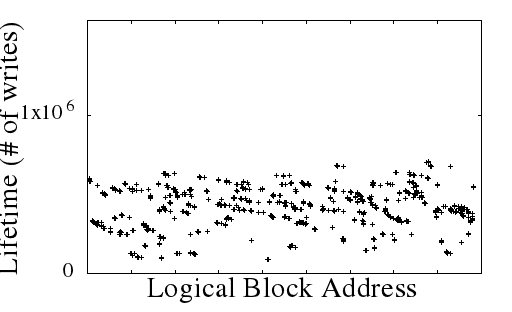
\includegraphics[width=0.2\textwidth]{figure/pcID_3}}
%\vspace{-7pt}
\caption{Data lifetime distributions of different PCs for an append-only workload.} 
\label{fig:types_and_PCs}
%\vspace{-20pt}
\end{figure}

To confirm our hypothesis that data lifetimes can be distinguished by tracking
dominant I/O activities and a PC is a useful hint to identify such I/O
activities, we have conducted a set of experiments with RocksDB using two
different methods.  First, we manually identify dominant I/O activities by
inspecting the source code.  Second, we automatically detect dominant I/O
activities by extracting PCs for write-related system functions.
Fig.~\ref{fig:types_and_PCs} shows our experimental results.  As shown in
Figs.~\ref{fig:types_and_PCs}(a) and (c), data written by logging and flushing
activities have distinct lifetimes; while logging data have short lifetimes,
data flushed by RocksDB are likely to have much longer lifetimes.
Figs.~\ref{fig:types_and_PCs}(b) and (d) also show similar patterns as
Figs.~\ref{fig:types_and_PCs}(a) and (c), which means that a PC can be used to
identify dominant I/O activities.

We have conducted additional experiments with SQLite and GCC which have
different I/O characteristics from RocksDB. In contrast to RocksDB that writes
almost all of the data in an append-only manner, SQLite and GCC write data or
result files in place. Fig.~\ref{fig:updating_PCs} are our experimental results
which show distinct lifetime distributions of I/O activities of SQLite and GCC.
As shown in Figs.~\ref{fig:updating_PCs}(a) and (b), the logging activity of
SQLite generates short-lived data.  This is because SQLite overwrites logging
data in a small and fixed storage space and then removes them soon.  We also
see that the logging activity is successfully identified by PCs. Similarly,
lifetime distribution of temporary files created by GCC are also relatively
short as shown in Fig.~\ref{fig:updating_PCs}(c) and (d). We observe that GCC
instances are forked and terminated, generating temporary files, but all those
activities are captured by PCs. \textcolor{red}{(TODO: 수명이 긴 경우도
보여주면 좋을 듯...)}


\begin{figure}[t]
\centering
\hfill
%\vspace{-10pt}
	\subfloat[SQLite: log (PC)]{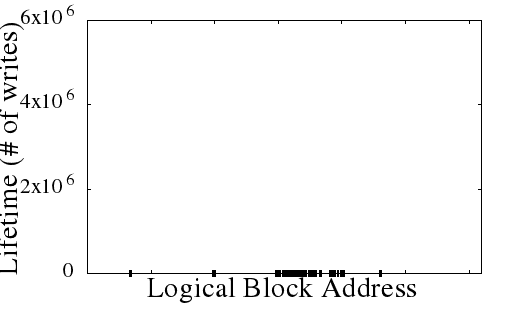
\includegraphics[width=0.2\textwidth]{figure/sqlite_short_LBA}} % data from py-tpcc/4/09151534
	\hspace{2pt}
	\subfloat[SQLite: log (manual)]{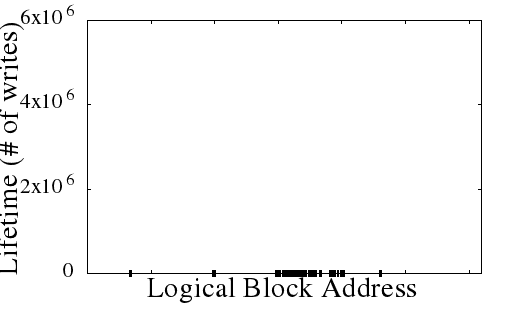
\includegraphics[width=0.2\textwidth]{figure/sqlite_short_LBA_manual}}
\hfill
\vspace{7pt}
	\subfloat[gcc: temp files (PC)] {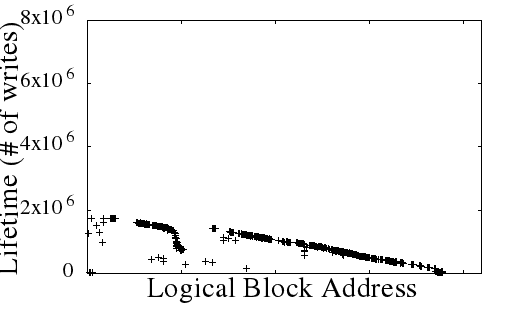
\includegraphics[width=0.2\textwidth]{figure/compile_short_PC}} % data from 08231319
	\hspace{2pt}
	\subfloat[gcc: temp files (manual)]{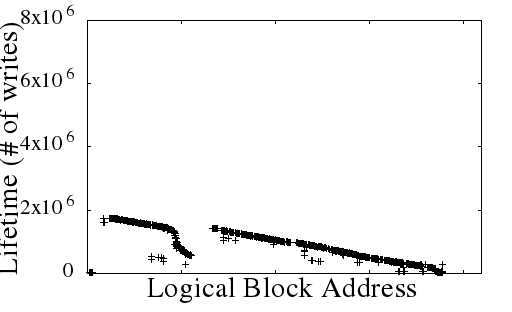
\includegraphics[width=0.2\textwidth]{figure/compile_short_manual}}
%\vspace{-7pt}
\caption{Data lifetime distributions of different PCs for updating workloads.} 
\label{fig:updating_PCs}
%\vspace{-20pt}
\end{figure}


\subsection{Extracting PCs}
As mentioned earlier, \textcolor{red}{a PC signature (처음 등장???)} is defined
to be the sum of program counters along the execution path of function calls
that finally reaches a write-related system function.  In theory, program
counter values in the execution path can be extracted in a relatively
straightforward manner.  Except for inline functions, every function call
involves pushing the address of the next instruction of a caller as a return
address to the stack, followed by pushing a frame pointer value.  By referring
to frame pointers, we are able to back-track stack frames of a process and
selectively get return addresses for generating a PC signature.
\textcolor{red}{(TODO: 그림위치를 변경할 필요가 있음. (a)를 이전 절로 이동?)For
example, Fig.~\ref{fig:getpc}(b) illustrates a stack of RocksDB corresponding
to Fig.~\ref{fig:getpc}(a), where return addresses are pushed before calling
the \textsf{\small  write()}, \textsf{\small AddRecord()} and \textsf{\small
WriteToWAL()} functions.}  Since frame pointer values in the stack hold the
addresses of previous frame pointers, we can easily obtain return addresses and
accumulate them to compute a PC signature.  

%For example,
%Fig.~\ref{fig:getpc}(a) shows abstracted execution paths of log data and
%compaction data in RocksDB.  The return addresses are pushed before calling the
%\textsf{\small  write()}, \textsf{\small AddRecord()} and \textsf{\small
%WriteToWAL()} functions.  Fig.~\ref{fig:getpc}(b) illustrates how a PC
%signature is obtained by back-tracking the stack.  Since frame pointer values
%in the stack hold the addresses of previous frame pointers, we can easily
%obtain return addresses and accumulate them to compute a PC signature.  

The frame pointer-based approach for computing a PC signature, however, is not
always possible because modern C/C++ compilers often do not use a frame pointer
for improving the efficiency of register allocation.  One example is a {\tt
-fomit-frame-pointer} option of GCC~\cite{GCC}.  This option enables to use a frame
pointer as a general-purpose register for performance, but makes it difficult for us
to back-track return addresses along the call chains.  

\begin{figure}[t]
%	\vspace{-10pt}
	\centering
	%\vspace{-8pt}
	\subfloat[Abstracted execution paths of two I/O activities of RocksDB.]{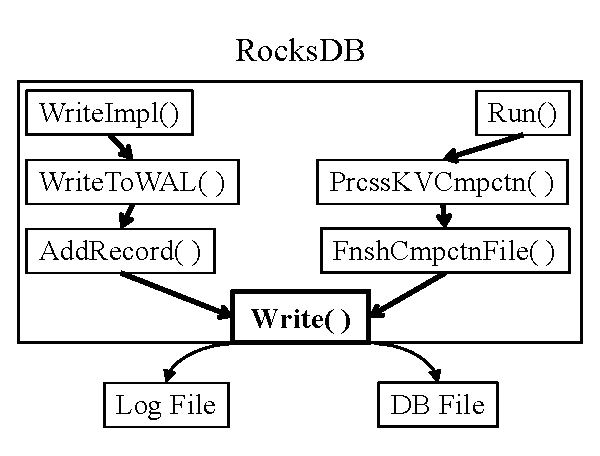
\includegraphics[width=0.3\textwidth]{figure/writepath}}  
	%\vspace{-14pt}
	\hfill
	\subfloat[with the frame pointer.]{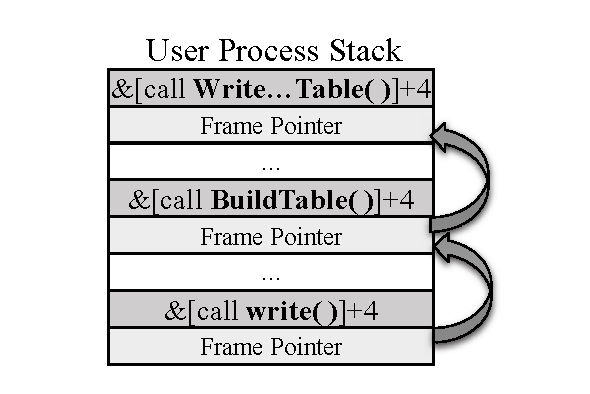
\includegraphics[width=0.22\textwidth]{figure/getpc_2}}
	\subfloat[without the frame pointer.]{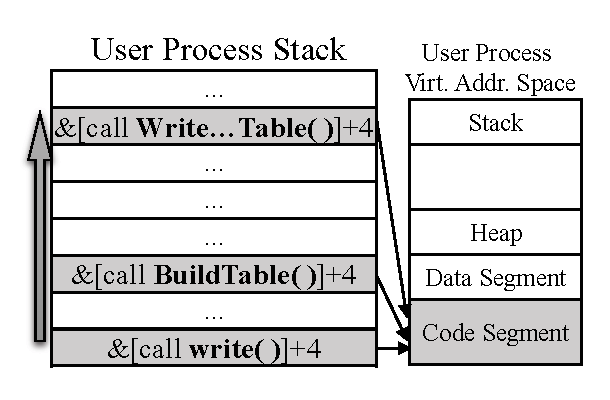
\includegraphics[width=0.22\textwidth]{figure/getpc_3}}
	%\vspace{-9pt}
	\caption{An example execution path and its PC extraction methods.}
	%\caption{An example execution path and its PC extraction.} %shane part
	\label{fig:getpc}
	%\vspace{-20pt}
\end{figure}

\textcolor{red}{\sout{The PC extractor of \textsf{\small PCStream} employs a simple but effective}}
We employ a simple but effective workaround for back-tracking a call stack when
a frame pointer is not available.  When a write system call is made,
\textcolor{red}{\sout{the PC extractor} (처음나옴???)} we scan every word in the stack
and checks if it belongs to process's code segment.  If the scanned stack word
holds a value within the address range of the code segment, it assumes that it
is a return address.  Since scanning the entire stack takes too long, we stop
the scanning when a sufficient number of return address candidates are found.
In the current implementation, only five candidates are used for PC
computation.  Even though it is quite ad-hoc, this restricted scan is effective
in distinguishing different PCs; it is very unlikely that two different PCs
follow exactly the same execution path to the \textsf{\small write()} system
call.  In our evaluation with a 3.4 GHz CPU machine, the overhead of the
restricted scan was almost negligible, taking only 300-400 $n$sec per
\textsf{\small write()} system call.




